% =====================================================================
%  The Silent Tax: How Typos Reshape Reasoning in Thinking LLMs
%  Final report -- ACL format (acl.sty, final mode).
%
%  Provenance:
%    Author text from report_text.txt (re-synced 2026-09-19), revised on
%    branch review/report-fixes (2026-09-22): ACL template, length cut to
%    the 8-page limit, numeric corrections, findings added to the
%    Introduction, Conclusion moved before Limitations; related work and
%    bibliography verified against sources (2026-09-23). report_text.txt
%    must be updated to match before verify_text.py is run again.
%    3 Method: taken from Ron's paper.
%
% =====================================================================
\documentclass[11pt]{article}

\usepackage[final]{acl}
\usepackage{times}
\usepackage{latexsym}
\usepackage[T1]{fontenc}
\usepackage[utf8]{inputenc}
\usepackage{microtype}
\usepackage{inconsolata}
\usepackage{booktabs}
\usepackage{graphicx}
\usepackage{amsmath}
\usepackage{amssymb}
\usepackage{float}
% stfloats lets a full-width figure*/table* sit at the BOTTOM of a page as well
% as the top, so wide floats stay near the text that cites them.
\usepackage{stfloats}

% Float placement only (no spacing changes): let floats take more of a page
% before LaTeX defers them to a float-only page.
\renewcommand{\topfraction}{0.9}
\renewcommand{\bottomfraction}{0.7}
\renewcommand{\textfraction}{0.08}
\renewcommand{\floatpagefraction}{0.75}
\renewcommand{\dbltopfraction}{0.9}
\renewcommand{\dblfloatpagefraction}{0.75}

\newcommand{\pp}{\,pp}
\newcommand{\arrow}{$\rightarrow$}

\title{The Silent Tax: How Typos Reshape Reasoning in Thinking LLMs}

\author{
Shiran Hamami \\ 207487026 \\ \texttt{shiranhamami@mail.tau.ac.il} \And
Dolev Abudi \\ 323096099 \\ \texttt{dolevabudi@mail.tau.ac.il} \AND
Ron Shtricker \\ 209524552 \\ \texttt{ronshtricker@mail.tau.ac.il} \And
Ido Azoulay \\ 212710958 \\ \texttt{idoazoulay1@mail.tau.ac.il}
}

\begin{document}
\maketitle

% ---------------------------------------------------------------------
\begin{abstract}
Reasoning models perform strongly on clean mathematical and scientific
benchmarks, but real users often write with typos. We study how these everyday
errors affect not only final-answer accuracy, but also the reasoning process
itself. We introduce a controlled typo generator that independently varies the
number of corrupted words and the proportion of typos that produce another
valid English word, apply it to 500 questions from each of GSM8K, MATH-500 and
ARC-Challenge, and evaluate DeepSeek-R1-Distill-Qwen-7B across all corruption
settings. Typos consistently reduce accuracy, most on GSM8K, where it falls from
91.4\% on clean questions to 60.4\% in the most corrupted setting. Typos that
produce another valid word are more harmful than non-word typos: depending on
the dataset, a real-word typo is estimated to be 1.3 to 5.3 times more damaging
per typo. The reasoning traces show that the model often notices that something
is wrong, with longer reasoning and more uncertainty language, but this does not
translate into more effective self-correction: the model hesitates more, but
does not verify more. None of the lightweight mitigations we tested (a typo
warning, rewriting the question first, or an external spell checker)
consistently improved accuracy. The main challenge is not detecting that the
input is corrupted, but recovering its intended meaning.
\end{abstract}

% =====================================================================
\section{Introduction}
% =====================================================================

Chain-of-thought prompting and reasoning-focused models have substantially
improved performance on mathematical and scientific benchmarks
\citep{wei2022,deepseekr1}. However, benchmark questions are carefully written,
while real users often make simple typing mistakes such as swapped letters,
missing characters, or nearby-key errors. Strong performance on clean benchmark
text may therefore overestimate reliability in real-world use.

Previous work has shown that typos can hurt LLM performance
\citep{gan2024,zhao2026}, partly because they disrupt subword tokenization
\citep{chai2024}. However, these
studies mainly focus on final-answer accuracy and do not examine what happens
inside the reasoning process.

Reasoning models make this question especially interesting. Their long reasoning
traces give them many opportunities to notice a corrupted word, infer what was
intended, and recover before producing the final answer. Do they actually do so?

To study this, our typo generator separates two factors: how many words are
corrupted and what kind of corruption they contain. In particular, we vary the
share of typos that accidentally produce another valid English word. This allows
us to compare real-word and non-word typos while keeping the total number of
typos fixed and using the same questions in every condition, a comparison that,
to our knowledge, previous LLM typo studies have not made. We evaluate
DeepSeek-R1-Distill-Qwen-7B \citep{deepseekr1} across the full set of conditions
on three datasets with different reasoning characteristics, and examine the
reasoning traces themselves using word-level alignment and an LLM judge.

Our main contributions are: (i) a controlled experimental setup that
independently varies typo rate and the proportion of real-word typos across
three datasets; (ii) an analysis of how typos affect the reasoning process
itself, including model uncertainty, whether the model notices corrupted words,
and whether it repairs them; and (iii) an evaluation of three simple mitigation
strategies: warning the model that the input may contain typos, asking it to
correct possible typos before solving the problem, and applying an external
spell checker before the model sees the question.

Our main findings are as follows. Typos cost up to 31 percentage points of
accuracy on GSM8K, and the loss comes from wrong answers rather than truncated
generations (\S\ref{sec:acc}). At a fixed number of typos, real-word typos are
more harmful than non-word ones, by 1.3--5.3$\times$ per typo
(\S\ref{sec:realword}). Contrary to our initial expectation that real-word
typos would pass unnoticed, the model flags corrupted words, and hedges, more
often as corruption grows, yet it also misreads more words and does not verify
more (\S\ref{sec:repair}, \S\ref{sec:doubt}). Finally, none of the three
mitigations reliably recovers the loss (\S\ref{sec:fixes}).

\begin{figure}[tbp]
\centering
\footnotesize
\setlength{\fboxsep}{4pt}
\fbox{\begin{minipage}{0.94\columnwidth}
\textbf{Clean} (model answers 18, correct)

\smallskip
\noindent\emph{Janet's ducks lay 16 eggs per day. She eats three for breakfast
every morning and bakes muffins for her friends every day with four. She sells
the remainder at the farmers' market daily for \$2 per fresh duck egg. How much
in dollars does she make every day at the farmers' market?}

\medskip\hrule\medskip

\textbf{$r{=}25\%$, $\rho{=}40\%$} (model answers 26, wrong)

\smallskip
\noindent\emph{Janet's \textbf{duck} lay 16 eggs per \textbf{adqy}.
\textbf{Sje} \textbf{east} \textbf{rthere} for breakfast every morning and bakes
muffins for \textbf{uher} \textbf{friend} every \textbf{azy} with four. She
sells the remainder at the farmers' market daily for \$2 per \textbf{resh} duck
egg. How much in dollars does she make every day at the \textbf{faremrs'}
market?}
\end{minipage}}
\caption{A single GSM8K item under our generator. Numbers and \LaTeX{} are
protected; only alphabetic words are corrupted. Three of the ten typos are
\emph{real words} (\texttt{eats\arrow east}, \texttt{ducks\arrow duck},
\texttt{friends\arrow friend}) and are invisible to a spell checker. The model
answers 26 instead of 18.}
\label{fig:example}
\end{figure}

% =====================================================================
\section{Background and Related Work}
% =====================================================================

\paragraph{Sensitivity to character-level typos.}
\citet{belinkov2018} show that both synthetic and natural character-level noise
degrade neural machine translation, and that robustness to one type of noise
does not transfer to others. Small adversarial character- and word-level edits
also fool text classifiers \citep{ebrahimi2018,jin2020} and degrade LLMs through
their prompts \citep{zhu2024}. Two lines of defense mirror our mitigations:
\citet{pruthi2019} place a word-recognition model in front of the classifier to
undo adversarial misspellings, and \citet{wang2024noisy} find that having an LLM
clean a noisy instruction before the task is difficult, particularly for
open-source models.

\paragraph{Typos and modern LLMs.}
\citet{gan2024} use an optimized adversarial search to inject typos into
reasoning benchmarks such as GSM8K, BBH, and MMLU, and show that model accuracy
drops substantially as the number of character-level errors increases.
\citet{chai2024} show that character-level typos can hurt model performance
partly because they change how words are split into subwords.
\citet{zhao2026} study typo robustness across 12 languages and 18 open-source
models, and find that typos hurt most on tasks that require generation or
reasoning. Concurrently, \citet{hu2026hive} report that a thinking budget
recovers most of the accuracy lost to QWERTY keyboard perturbations, and trace
the harm to how many of the question's tokens are destroyed.

These studies mainly measure final-answer accuracy rather than the reasoning
process itself, and they vary typos by generation mechanism rather than by
whether the corrupted form is itself a valid word. That distinction is classic
in spelling correction, where real-word errors cannot be caught by dictionary
lookup \citep{kukich1992,hirst2005}, and it matters here too. A typo that
creates a non-word, such as \texttt{triangle\arrow trianlge}, mainly disrupts
tokenization, while a typo that creates another valid word, such as
\texttt{sum\arrow sun}, is tokenized normally but changes the meaning of the
sentence. Our study separates these cases and examines how the model responds
to each during reasoning.

\paragraph{Reasoning traces and self-correction.}
Reasoning models such as DeepSeek-R1 \citep{deepseekr1} produce long reasoning
traces before giving a final answer. These traces do not always fully reflect
the model's internal reasoning \citep{turpin2023}, and LLMs often struggle to
correct their own reasoning without external feedback, sometimes even degrading
their answers in the process \citep{huang2024}. Our setting asks a related but
different question: can a long reasoning process help the model deal with errors
that are already present in the input? A typo may be detectable from context,
giving the model an opportunity to notice it, infer the intended word, and
continue reasoning correctly.

% =====================================================================
\section{Method}
% =====================================================================

\subsection{Controlled typo generation}

We generate corrupted versions of each question by modifying only its
natural-language text, building on the keyboard-aware edit operations of
MulTypo \citep{zhao2026} and adding control over real-word typos. Numbers, \LaTeX{} expressions, and \LaTeX{} command
names are protected and never modified. Candidate words must consist only of
ASCII letters, and we exclude single-character words and a small set of common
function words.

The generator varies two factors independently. The typo rate $r$ determines
how many eligible words are corrupted, while the real-word ratio $\rho$
determines the target fraction of those corruptions that should result in
another valid English word. For example, \texttt{eats}~\arrow~\texttt{east}
is a real-word typo, while \texttt{ducks}~\arrow~\texttt{dcks} is a non-word
typo. Words are selected for corruption before $\rho$ is applied, so for a
fixed typo rate the number of corrupted words is identical across all values
of $\rho$.

Each corrupted word receives a character-level edit sampled with weights 0.40
adjacent-key substitution, 0.20 deletion, 0.20 insertion, and 0.20
transposition. With probability 0.10, a second edit is applied to the same
word.

For each question, we convert $\rho$ into a target number of real-word typos,
using probabilistic rounding when the target is not an integer. We then process
the selected words in random order. While the target has not been reached, the
generator searches for valid real-word variants using the NLTK English lexicon
\citep{bird2009nltk}.
If none exists for a selected word, that word receives a non-word typo and the
generator continues trying to satisfy the target with the remaining words. Any
real word produced accidentally is counted toward the target. Because the
selected words are not chosen based on whether a real-word variant exists, the
requested ratio cannot always be reached exactly; the generator then gets as
close to the target as the selected words allow.
Table~\ref{tab:datastats} reports the achieved ratios.

For each benchmark, we create a clean condition that is identical to the
original dataset, together with nine corrupted conditions. These combine typo
rates $r \in \{25, 50, 75\}\%$ with real-word ratios
$\rho \in \{10, 40, 70\}\%$. The generator is seeded consistently across
conditions, and the same questions are used in every condition, allowing direct
paired comparisons. The resulting dataset variants are available on the Hugging
Face Hub.

\subsection{Datasets}

We use 500 questions from each of three benchmarks: GSM8K \citep{cobbe2021},
MATH-500 \citep{hendrycks2021,lightman2024}, and ARC-Challenge
\citep{clark2018}. They differ in how much of the information needed to solve a
question is expressed in natural-language text. GSM8K contains arithmetic word
problems whose structure is described almost entirely in prose, and its
questions are relatively long. MATH-500 contains shorter competition problems
with substantial \LaTeX{} content, which our generator protects. ARC-Challenge
contains short multiple-choice science questions, whose answer options may help
the model interpret a corrupted question.

As a result, the same typo rate does not produce the same absolute number of
typos across datasets: GSM8K receives the most corruption per question
(Table~\ref{tab:datastats}). We therefore compare corruption levels within each
dataset rather than across benchmarks.

\begin{table}[tbp]
\centering
\footnotesize
\setlength{\tabcolsep}{3.5pt}
\begin{tabular}{lrrr}
\toprule
 & GSM8K & MATH-500 & ARC-C \\
\midrule
questions & 500 & 500 & 500 \\
mean words per question & 45.8 & 31.5 & 23.5 \\
median words per question & 43 & 26 & 20 \\
eligible words per question & 30.6 & 15.7 & 16.6 \\
\midrule
typos per question, $r{=}25\%$ & 7.6 & 4.0 & 4.2 \\
typos per question, $r{=}50\%$ & 15.3 & 7.9 & 8.3 \\
typos per question, $r{=}75\%$ & 22.9 & 11.8 & 12.4 \\
\midrule
achieved real-word ratio, $\rho{=}10\%$ & 0.100 & 0.099 & 0.102 \\
achieved real-word ratio, $\rho{=}40\%$ & 0.399 & 0.397 & 0.401 \\
achieved real-word ratio, $\rho{=}70\%$ & 0.698 & 0.681 & 0.682 \\
\midrule
total corrupted words & 68{,}739 & 35{,}685 & 37{,}248 \\
\bottomrule
\end{tabular}

\caption{Dataset and corruption statistics over the nine corrupted conditions
($r\in\{25,50,75\}\%$, $\rho\in\{10,40,70\}\%$), first 500 questions of GSM8K
and ARC-Challenge and all of MATH-500. \emph{Eligible words} are those the
generator may corrupt, after protected spans, single-character words and
function words are removed; the typo rate applies to them, and real-word ratios
are pooled over all corrupted words.}
\label{tab:datastats}
\end{table}

% =====================================================================
\section{Experimental Setup}
\label{sec:setup}
% =====================================================================

\paragraph{Models.}
We use DeepSeek-R1-Distill-Qwen-7B \citep{deepseekr1}, accessed through the
Hugging Face API, with temperature 0.6 and top-$p$ 0.95 (the model-card
defaults, to reflect how a typical user would run it) and one response per
question. The maximum generation length is 20{,}000 tokens for GSM8K and
17{,}000 for MATH-500 and ARC-Challenge, which we found sufficient for the model
to finish on a large majority of questions. For the LLM-based evaluation we use
Llama-3.3-70B-Instruct \citep{llama3}, also through the Hugging Face API, with
temperature 0.

\paragraph{Prompts.}
For math problems, we provide the question followed by the instruction:
``Please reason step by step, and put your final answer within
\texttt{\textbackslash boxed\{\}}.'' For multiple-choice questions, we present
the four answer options with shuffled labels and ask the model to return the
final answer as a boxed letter. Typos are added only to the question itself,
while the instruction remains unchanged and typo-free.

\paragraph{Scoring.}
We extract the final answer only from the text produced after the closing
\texttt{</think>} tag. Responses that reach the token limit without producing a
final answer are marked as unanswered. GSM8K is evaluated using normalized
numeric matching, MATH-500 using symbolic equivalence with
\texttt{math\_verify}, and ARC using exact answer-letter matching. We report
accuracy over answered questions together with the number of answered
responses, and check the effect of truncation with strict accuracy, which
counts unanswered responses as wrong.

\paragraph{Statistics.}
Since each condition contains the same 500 questions, we use paired tests. We
count the questions that change from correct to incorrect and from incorrect to
correct, and compare these paired outcomes with a continuity-corrected McNemar
test, which separates the effect of typos from differences in question
difficulty. Tables report uncorrected $p$-values; in the text we also state
which results survive a Holm correction over the nine tests of each family
within a dataset.

\paragraph{Reasoning trace analysis.}
We analyze the reasoning traces in three ways. First, word-level alignment
tracks how the model handles each corrupted word: whether the trace uses the
original word, the corrupted form, or both, classifying each typo as silently
fixed, flagged, misread, or not used (\S\ref{sec:repair}). Second, we count
curated uncertainty and second-guessing expressions, normalized by trace length
(\S\ref{sec:doubt}). Third, an LLM judge \citep{zheng2023} receives the list of corrupted words
with their originals, the question as shown to the model, and the reasoning
trace (its first and last 2{,}000 characters). Using a fixed rubric, it assigns
a \emph{self-doubt} score from 0 (a clear, straight-line solution) to 10
(pervasive uncertainty, reversals or looping), and a \emph{repair} score from 0
(the intended meaning of the question is fully understood) to 5 (the model
reasons from the wrong meaning). Higher is worse on both scales. The judge
scores answered traces only.

% =====================================================================
\section{Results}
% =====================================================================

\subsection{Effect of typos on accuracy}
\label{sec:acc}

\begin{figure*}[tbp]
\centering
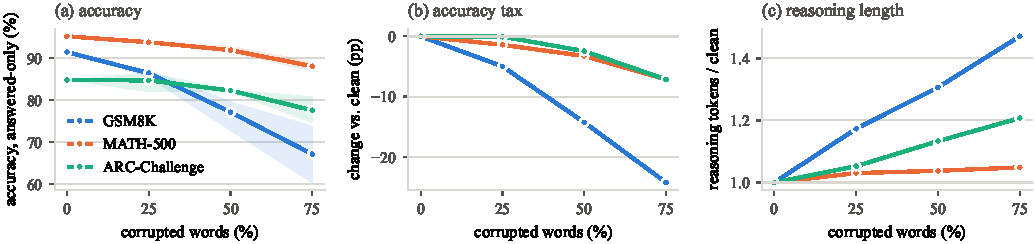
\includegraphics[width=\textwidth]{figures/fig_accuracy.pdf}
\caption{\textbf{The accuracy tax.} \emph{(a)} answered-only accuracy against
the typo rate; the line is the mean over the three real-word ratios and the band
spans them. \emph{(b)} the same as a change from clean, in percentage points.
\emph{(c)} mean generated tokens relative to clean. Accuracy falls with the typo
rate on all three datasets and falls fastest on GSM8K, where the text carries
the whole problem. On average, reasoning gets \emph{longer} under typos, so the
loss is not the model giving up early.}
\label{fig:accuracy}
\end{figure*}

Figure~\ref{fig:accuracy} and Table~\ref{tab:grid} in the appendix show the full
results. On GSM8K, answered-only accuracy drops from 91.4\% on clean questions
to 60.4\% in the most corrupted condition ($r{=}75$, $\rho{=}70$), a decrease of
31.0 percentage points. ARC drops from 84.7\% to 74.7\%, and MATH-500 from
95.2\% to 86.9\%. On all three datasets accuracy is lowest at the highest typo
rate, although on ARC the mildest rate ($r{=}25$) is still on par with clean.

The paired analysis shows the same trend. In the most corrupted GSM8K condition,
164 questions change from correct to incorrect, while only 14 change from
incorrect to correct, out of 480 questions answered in both conditions
($p < 10^{-6}$). ARC shows 75 correct-to-incorrect versus 26
incorrect-to-correct changes, and MATH-500 shows 46 versus 7, both
significant. After Holm correction, all nine GSM8K conditions remain
significant, against four on MATH-500 (all at $r \geq 50$) and two on ARC (both
at $r{=}75$). One possible explanation is how much each task depends on the
wording of the question: GSM8K problems rely on the text to describe the
quantities and relationships needed for the solution, ARC's answer options may
help the model recover some information, and much of the mathematical content
of MATH-500 is written in protected \LaTeX{}.

Truncation does not explain the loss. Counting unanswered responses as wrong,
GSM8K accuracy falls from 91.4\% to 58.0\%; of this strict drop at $r{=}75$,
$\rho{=}70$, 93\% comes from answered-but-wrong responses and only 7\% from
truncation, and on MATH-500 and ARC truncation contributes nothing. Typos also
lengthen the reasoning: on GSM8K the mean trace grows from 1,582 tokens on clean
questions to 2,306 in the most corrupted condition (and up to 2,594 at
$r{=}75$, $\rho{=}40$), with smaller increases on MATH-500 and ARC. Wrong
answers have longer traces than correct ones in every configuration, so
additional reasoning is associated with difficulty rather than with successful
recovery (Figure~\ref{fig:accuracy}c; Table~\ref{tab:support}).

\subsection{Real-word typos are more harmful}
\label{sec:realword}

\begin{figure}[tbp]
\centering
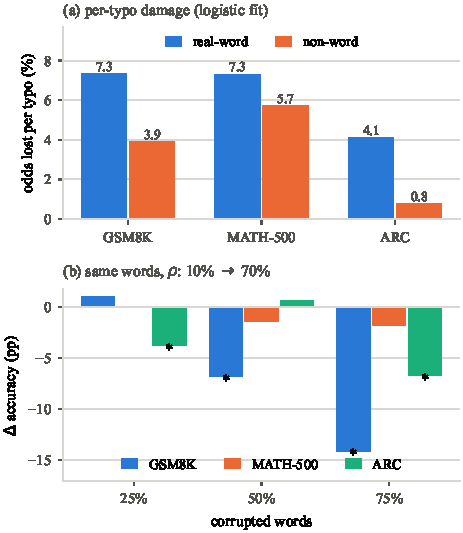
\includegraphics[width=\columnwidth]{figures/fig_realword.pdf}
\caption{\textbf{The real-word effect.} \emph{(a)} multiplicative loss in the
odds of a correct answer per additional typo, from a logistic regression fitting
real-word and non-word counts separately. \emph{(b)} the controlled paired
comparison: the same questions with the same number of typos, changing only the
real-word share from $\rho{=}10$ to $\rho{=}70$. $^{*}$ marks McNemar
$p<0.05$ (uncorrected).}
\label{fig:realword}
\end{figure}

Because typo rate and real-word ratio are varied independently, we can compare
real-word and non-word typos while controlling for the total number of typos.
For each dataset, we fit a logistic regression that predicts whether the final
answer is correct from the number of real-word and non-word typos
(Figure~\ref{fig:realword}a). An additional real-word typo has a stronger
negative association with correctness than an additional non-word typo: the
relative per-typo loss is about 1.9$\times$ larger on GSM8K, 1.3$\times$ on
MATH-500, and 5.3$\times$ on ARC (Table~\ref{tab:realword-logit}).

The paired comparisons support this pattern, although the effect depends on the
overall typo rate. On GSM8K at a 75\% typo rate, increasing the real-word share
from 10\% to 70\% lowers accuracy by 14.1 percentage points, even though the
same questions contain the same total number of typos. The difference is also
significant at a 50\% typo rate (both after Holm correction), but not at 25\%.
When corruption is mild, the model can often handle both kinds of typo, and the
difference becomes more pronounced as the overall typo rate increases
(Figure~\ref{fig:realword}b; Table~\ref{tab:realword-paired}). On ARC, the
effect is significant at $r{=}75$ ($-6.7$\pp{}, surviving correction); two
contrasts at $r{=}25$ reach $p<0.05$ but do not survive correction, and none at
$r{=}50$ does. MATH-500 shows no significant difference at any typo rate,
consistent with its smaller number of corrupted words.

Overall, real-word typos appear especially difficult for the model. Unlike
non-word typos, which produce visibly unusual word forms, they result in valid
words and can change the meaning of the input without creating an obvious
tokenization problem.

\subsection{Repair behavior: noticed but not repaired}
\label{sec:repair}

\begin{figure*}[tbp]
\centering
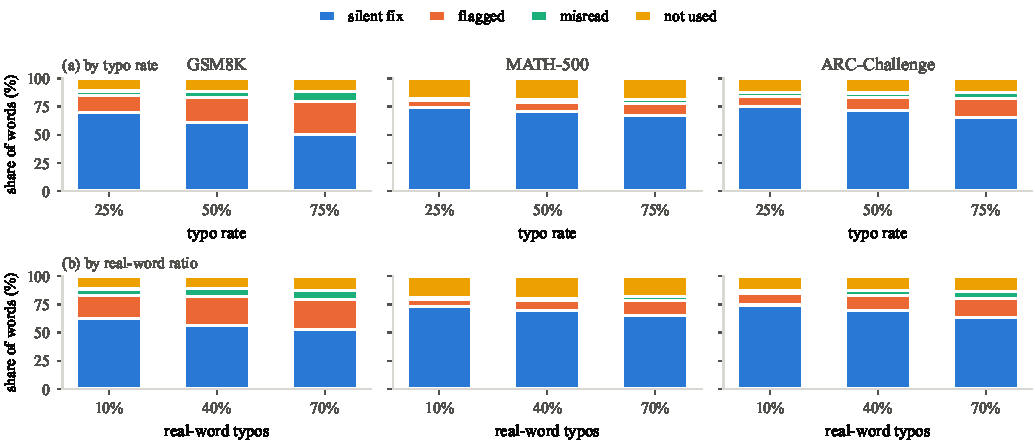
\includegraphics[width=\textwidth]{figures/fig_repair.pdf}
\caption{\textbf{Word-level repair behavior.} How every corrupted word is
handled in the reasoning trace. \emph{(a)} against the typo rate, pooled over
real-word ratios. \emph{(b)} against the real-word ratio, pooled over typo
rates. Silent fixing gives way to explicit flagging and to misreading as either
the typo rate or the real-word ratio increases, while the share of words never
referred to stays roughly constant. Per-configuration values are in
Table~\ref{tab:repair}.}
\label{fig:repair}
\end{figure*}

We recover each corrupted word by comparing the clean and corrupted versions of
the question, and classify how the model handles it in the reasoning trace:
\textbf{silent fix}, only the original word appears (the model recovered the
intended word without mentioning the typo); \textbf{flagged}, both the original
and the corrupted form appear (the model noticed and corrected the typo);
\textbf{misread}, only the corrupted form appears (the model took it as the
wrong word); and \textbf{not used}, neither form appears.

We originally expected real-word typos to go unnoticed more often, while
non-word typos would be easier to detect and correct explicitly. The results
only partly support this prediction. As the typo rate increases from 25\% to
75\%, silent fixing decreases on all three datasets; on GSM8K, for example, it
falls from 73.3\% to 55.8\% at $\rho{=}10$. At the same time, flagging and
misreading become more common: pooled over real-word ratios, misreading rises
from 4.0\% to 8.3\% on GSM8K and from 1.5\% to 2.9\% on MATH-500, and less
steeply on ARC, from 3.5\% to 5.1\% (Figure~\ref{fig:repair};
Table~\ref{tab:repair}).

Increasing the real-word ratio has a similar effect. Pooled across typo rates on
GSM8K, silent fixing falls from 62.3\% to 52.9\% as $\rho$ increases from 10 to
70, while flagging rises from 21.0\% to 26.8\% and misreading from 5.4\% to
7.7\%; the same overall pattern appears on MATH-500 and ARC. Misreading is also
related to failure: in every configuration it is 1.2 to 2.0 times more frequent
in GSM8K traces that end in a wrong answer, and 1.2 to 2.4 times on ARC; on
MATH-500, where misreads are rare, the relation is not consistent
(Table~\ref{tab:repair}). The share of typos that are not used stays stable
within each dataset but differs across tasks, roughly 12\% on GSM8K, 13\% on
ARC, and 19\% on MATH-500, possibly because MATH-500 reasoning is more symbolic
and refers back to the wording of the question less often.

The judge's repair score (\S\ref{sec:setup}; Table~\ref{tab:judge}) tells the
same story. It rises with the typo rate, and wrong answers score higher than
correct ones (2.30 vs.\ 0.87 on GSM8K), linking misunderstanding of the
corrupted question to failure. It also rises with the real-word ratio in every
dataset and typo-rate cell, consistent with real-word typos being harder to
repair, although we did not test this trend for significance.

\subsection{Self-doubt}
\label{sec:doubt}

\begin{table}[tbp]
\centering
\footnotesize
\begin{tabular}{l rr rr rr}
\toprule
& \multicolumn{2}{c}{\textbf{GSM8K}} & \multicolumn{2}{c}{\textbf{MATH-500}} & \multicolumn{2}{c}{\textbf{ARC-C}} \\
\cmidrule(lr){2-3}\cmidrule(lr){4-5}\cmidrule(lr){6-7}
\textbf{condition} & repair & doubt & repair & doubt & repair & doubt \\
\midrule
\multicolumn{7}{l}{\emph{clean}} \\
\quad --- & 0.13 & 4.50 & 0.03 & 3.66 & 0.03 & 4.69 \\
\midrule \multicolumn{7}{l}{\emph{by typo rate }$r$} \\
\quad 25\% & 0.88 & 4.86 & 0.35 & 3.90 & 0.97 & 5.12 \\
\quad 50\% & 1.27 & 5.12 & 0.35 & 3.98 & 1.03 & 5.31 \\
\quad 75\% & 1.74 & 5.64 & 0.48 & 4.01 & 1.35 & 5.63 \\
\midrule \multicolumn{7}{l}{\emph{by real-word ratio }$\rho$} \\
\quad 10\% & 1.14 & 5.21 & 0.32 & 3.87 & 0.94 & 5.33 \\
\quad 40\% & 1.32 & 5.29 & 0.39 & 4.03 & 1.10 & 5.27 \\
\quad 70\% & 1.42 & 5.12 & 0.47 & 3.99 & 1.31 & 5.45 \\
\midrule \multicolumn{7}{l}{\emph{by final answer}} \\
\quad correct & 0.87 & 4.69 & 0.27 & 3.75 & 0.88 & 4.94 \\
\quad wrong & 2.30 & 6.75 & 1.30 & 5.81 & 1.62 & 6.88 \\
\bottomrule
\end{tabular}
\caption{Mean LLM-judge scores over answered traces. \emph{repair} is the repair
score (0--5, higher means less of the intended meaning recovered); \emph{doubt}
is the self-doubt score (0--10, higher means more hesitation and looping).}
\label{tab:judge}
\end{table}

We measure self-doubt with two curated sets of expressions. The uncertainty set
contains hedges such as \emph{maybe}, \emph{perhaps}, \emph{possibly},
\emph{might be}, and \emph{not sure}; the second-guessing set captures explicit
reconsideration, such as \emph{wait}, \emph{actually}, \emph{reconsider},
\emph{let me recheck}, and \emph{double-check}. We report matches per 1,000
reasoning words.

Uncertainty increases as the input becomes more corrupted. On GSM8K, it rises
from 7.4 markers per 1,000 words on clean input to 12.3 at a 25\% typo rate and
18.7 at 75\%, with the real-word ratio held at 10\%. The same trend holds on
MATH-500 and ARC at the higher typo rates, although on ARC the mildest rate is
not above clean. At a fixed typo rate, a higher real-word ratio tends to add
further uncertainty (Figure~\ref{fig:doubt}; Table~\ref{tab:support}).

Second-guessing behaves differently. Its density rises only slightly on GSM8K,
not at all on MATH-500 and ARC, and stays roughly flat across typo rates and
real-word ratios. The number of second-guessing expressions per trace does grow,
but mostly because corrupted inputs produce longer traces. Typos thus make the
model express more uncertainty without making it reconsider its reasoning more
often.

The contrast is clearer when we separate correct and incorrect answers. For the
same configuration, uncertainty is consistently more frequent in traces that end
with a wrong answer: 1.6 to 2.1 times on GSM8K, with similar patterns on ARC and
MATH-500, while second-guessing differs much less (Table~\ref{tab:support}).
This relation is not unique to typos: even on clean GSM8K questions, incorrect
answers contain substantially more uncertainty language than correct ones.

The judge's self-doubt score (Table~\ref{tab:judge}) rises with the typo rate on
all three datasets, and typo traces score higher than clean ones everywhere. The
real-word ratio, however, shows no consistent direction: pooled over typo rates,
the score varies by less than 0.2 points on each dataset. The judge therefore
confirms that more corruption brings more hesitation but, unlike the marker
counts, does not register an additional effect of the kind of corruption.

\begin{figure*}[tbp]
\centering
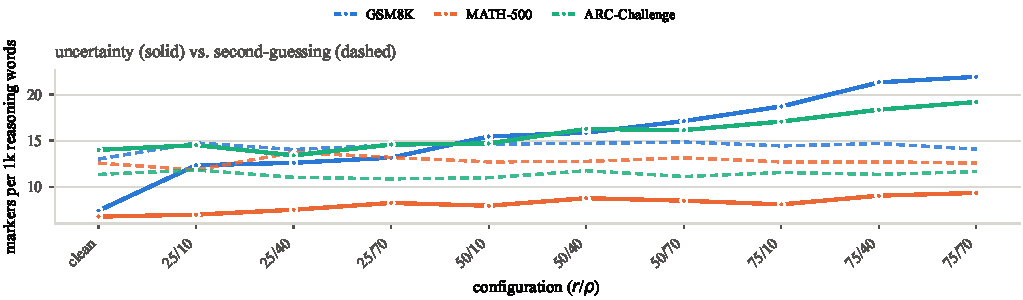
\includegraphics[width=\textwidth]{figures/fig_doubt.pdf}
\caption{\textbf{Self-doubt under typos.} Marker density per 1{,}000
reasoning words across the grid. Uncertainty markers (solid) rise with
corruption on all three datasets, most steeply on GSM8K, while second-guessing
markers (dashed) stay roughly flat: typos make the model express more doubt
without making it verify more. The same densities split by final answer are in
Table~\ref{tab:support}.}
\label{fig:doubt}
\end{figure*}

\subsection{No lightweight mitigation reliably helps}
\label{sec:fixes}

We tested the three mitigation strategies from our plan on GSM8K
(Table~\ref{tab:fixes}).

\paragraph{Warn.}
Prefixing the prompt with ``Note: the text may contain typos.'' changed
accuracy by only $-0.5$ percentage points on average across the nine typo
configurations, with effects ranging from $-4.3$ to $+3.5$ points. This is
consistent with \S\ref{sec:repair}, where the model often already showed signs
of noticing that the input was corrupted: the limitation does not appear to be
awareness of the typo itself.

\paragraph{Rewrite.}
Instructing the model to first rewrite the question with the typos corrected
and only then solve it performed worse than the original prompt in all nine
configurations, reducing accuracy by 4.7 percentage points on average and by up
to 7.5 points. Median reasoning length also fell, from about 1,300 to about 740
tokens (median over the nine typo configurations). One possible explanation is
that the rewrite step forces the model to commit to a single interpretation of
the corrupted question too early; if the reconstruction is wrong, the model
reasons about the wrong problem with little opportunity to recover.

\paragraph{Spell check.}
We applied an external spell checker (\texttt{pyspellchecker}, edit distance 2,
prose words only) to the same questions before sending them to the model. A
typo counts as recovered only if it is restored exactly to the original word.
Recovery dropped as the share of real-word typos increased: from 54.9\% at
$\rho{=}10$ to 39.9\% at $\rho{=}40$ and 25.8\% at $\rho{=}70$. This lexical
recovery did not translate into a consistent accuracy gain: the spell checker
changed accuracy by $-0.1$ percentage points on average, improving five
conditions and hurting four, with 62.2\% in the hardest condition. Spell
checkers detect non-word errors far better than real-word substitutions, and
may even replace a non-word typo with a wrong valid word, creating the kind of
error that \S\ref{sec:realword} found to be more harmful.

\begin{table}[tbp]
\centering
\footnotesize
\setlength{\tabcolsep}{4pt}
\begin{tabular}{lr rr rr rr}
\toprule
& \textbf{no fix} & \multicolumn{2}{c}{\textbf{warn}} & \multicolumn{2}{c}{\textbf{rewrite}} & \multicolumn{2}{c}{\textbf{spell check}} \\
\cmidrule(lr){3-4}\cmidrule(lr){5-6}\cmidrule(lr){7-8}
\textbf{$r$/$\rho$} & acc & acc & $\Delta$ & acc & $\Delta$ & acc & $\Delta$ \\
\midrule
25/10 & 85.5 & 85.7 & +0.2 & 83.8 & -1.7 & 87.0 & +1.5 \\
25/40 & 87.0 & 87.2 & +0.2 & 82.9 & -4.1 & 86.1 & -0.9 \\
25/70 & 86.7 & 85.5 & -1.2 & 80.2 & -6.6 & 85.3 & -1.4 \\
50/10 & 79.6 & 79.4 & -0.2 & 76.3 & -3.3 & 79.0 & -0.6 \\
50/40 & 79.0 & 74.7 & -4.3 & 71.5 & -7.5 & 75.0 & -4.0 \\
50/70 & 72.8 & 74.0 & +1.2 & 67.9 & -4.9 & 73.2 & +0.4 \\
75/10 & 73.8 & 70.6 & -3.2 & 66.9 & -6.9 & 75.3 & +1.5 \\
75/40 & 67.3 & 66.3 & -0.9 & 63.8 & -3.5 & 68.1 & +0.9 \\
75/70 & 60.4 & 63.9 & +3.5 & 56.9 & -3.5 & 62.2 & +1.8 \\
\midrule \textbf{mean} & & & \textbf{-0.5} & & \textbf{-4.7} & & \textbf{-0.1} \\
\bottomrule
\end{tabular}
\caption{GSM8K answered-only accuracy (\%) under each mitigation, per
configuration, with the change against the unmodified prompt (\emph{no fix}).
The mean row is taken over the nine typo configurations.}
\label{tab:fixes}
\end{table}

% =====================================================================
\section{Discussion}
% =====================================================================

The most consistent finding across our analyses is that real-word typos are more
harmful than non-word typos, in the per-typo regression, the paired comparisons,
and the spell-checker results. One might expect the opposite, since non-word
typos disrupt tokenization. Our results suggest that a non-word typo is visibly
unusual and signals that something is wrong, whereas a real-word typo is fluent,
tokenized normally, and may fit the sentence well enough that its wrong meaning
is taken at face value. The same property makes it hard for dictionary-based
correction, which can only act on forms that are not valid words.

The trace analysis points to a related conclusion. The model often notices that
the input is unusual: uncertainty language increases, corrupted words are
flagged more often, and traces become longer. This additional effort does not
reliably lead to recovery, which also explains why the mitigations had little
effect: a warning adds information the model often already has, while a forced
rewrite commits it early to a single, possibly wrong, interpretation. The main
difficulty is therefore not detecting that a typo exists, but recovering the
intended word when the corruption is ambiguous. A more promising direction may
be to keep multiple interpretations open during reasoning and resolve them
later using the structure of the problem. This is consistent with the concurrent
finding that a thinking budget absorbs most keyboard noise \citep{hu2026hive}:
in our data, too, the mildest typo rate costs little on MATH-500 and ARC. Dense
corruption and real-word typos are where long reasoning stops recovering.
Finally, longer traces should not be read as evidence of successful
self-correction: incorrect answers produce longer traces even on clean input.

% =====================================================================
\section{Conclusion}
% =====================================================================

Typos have a clear and consistent effect on reasoning performance. On GSM8K,
accuracy dropped by as much as 31 percentage points, with larger declines as the
corruption rate increased, and the strongest effect came from typos that turned
one valid English word into another. The main problem is not that the model
fails to notice corrupted input: it often recognizes that something is wrong,
but cannot reliably recover the intended meaning. Its traces show more
uncertainty rather than more verification, and neither prompting strategies nor
dictionary-based correction consistently improved performance. Robustness to
everyday typing errors should therefore be treated as a capability to be
developed explicitly, rather than assumed from strong benchmark performance.

All code is available in the project repository, and the raw generation logs are
hosted on the Hugging Face Hub (\texttt{ronshtricker/typo-reasoning-results}).
All reported results can be reproduced by running \texttt{download\_data.py}
followed by \texttt{run\_all.py}.

% =====================================================================
\section*{Limitations}
% =====================================================================

\paragraph{One model, one sample.}
All headline results come from a single 7B reasoning model at one decoding
setting with $n{=}1$ sample per question. Our plan called for several samples per
question, but the API budget did not permit it, so we cannot separate typo
effects from decoding variance at the level of an individual question. The
overall effects are much larger than expected sampling noise (McNemar
$p < 10^{-6}$ on $n{=}480$ paired items), but generalization to larger reasoning
models is untested.

\paragraph{Dataset substitution.}
We originally planned to use GPQA-Diamond \citep{rein2024}, but replaced it with ARC-Challenge,
which is also a multiple-choice science dataset. On clean GPQA-Diamond, the
model reached only about 52\% accuracy. Since random guessing gives 25\%, this
leaves limited room to measure further drops under corruption: as performance
gets closer to chance, changes in accuracy become harder to interpret as
reasoning failures rather than guessing. ARC-Challenge is easier and its answer
options may help the model recover some information, so our multiple-choice
results may underestimate the effect of typos on harder science questions.

\paragraph{Scope of the mitigation study.}
We tested the three mitigation methods only on GSM8K because the experiments
required additional paid API calls and our budget was limited. We chose GSM8K
because it showed the clearest drop in answer quality under typo corruption,
making it the most informative dataset for evaluating whether these mitigation
strategies could recover performance.

% =====================================================================
\section*{AI Disclosure and Reflection}
% =====================================================================

\paragraph{What we used AI for.}
We used GitHub Copilot with Claude primarily to support coding tasks during the
project. It helped us build the typo-generation and inference pipelines, write
analysis scripts, generate matplotlib code for figures, and improve the wording
of some parts of the paper. All methodological and experimental decisions,
including the two-axis corruption grid, typo-type weights, answer-extraction
rules, and judge rubric, were made by us. The analysis scripts were written with
Claude's assistance based on these decisions, and all reported results were
generated from the raw generation logs using those scripts.

\paragraph{Reflection.}
AI tools were especially useful for speeding up repetitive coding and analysis
tasks and for keeping the implementation consistent across experiments. However,
generated code and outputs still required careful checking, particularly for
numerical results. We therefore verified reported results against the raw data
and used a consistent scoring procedure throughout the analysis. Overall, the
project highlighted the importance of reproducibility and independent
verification when AI tools are used in research.

% =====================================================================
\bibliography{custom}
\bibliographystyle{acl_natbib}

% =====================================================================
\appendix
\clearpage
\onecolumn
\raggedbottom
\section*{Appendix}
\vspace{0.5em}
\renewcommand{\thetable}{A\arabic{table}}
\setcounter{table}{0}
\setlength{\tabcolsep}{2.6pt}

% =====================================================================

\begin{table}[H]
\centering
\scriptsize
\begin{tabular}{l rrrrrr rrrrrr rrrrrr}
\toprule
& \multicolumn{6}{c}{\textbf{GSM8K}} & \multicolumn{6}{c}{\textbf{MATH-500}} & \multicolumn{6}{c}{\textbf{ARC-Challenge}} \\
\cmidrule(lr){2-7}\cmidrule(lr){8-13}\cmidrule(lr){14-19}
\textbf{config} & acc & $n_a$ & tok & r$\to$w & w$\to$r & $p$ & acc & $n_a$ & tok & r$\to$w & w$\to$r & $p$ & acc & $n_a$ & tok & r$\to$w & w$\to$r & $p$ \\
\midrule
clean & 91.4 & 500 & 1582 & -- & -- & -- & 95.2 & 496 & 2927 & -- & -- & -- & 84.7 & 485 & 1172 & -- & -- & -- \\
typo25\_real10 & 85.5 & 497 & 1912 & 48 & 19 & 6.2e-04 & 93.9 & 495 & 2945 & 12 & 7 & 0.359 & 86.5 & 487 & 1222 & 24 & 31 & 0.418 \\
typo25\_real40 & 87.0 & 500 & 1814 & 40 & 18 & 0.006 & 93.4 & 498 & 3111 & 15 & 9 & 0.307 & 85.6 & 486 & 1246 & 28 & 33 & 0.609 \\
typo25\_real70 & 86.7 & 497 & 1843 & 43 & 19 & 0.003 & 93.9 & 494 & 2992 & 15 & 9 & 0.307 & 82.0 & 489 & 1234 & 42 & 26 & 0.069 \\
typo50\_real10 & 79.6 & 500 & 2024 & 78 & 19 & $<$1e-6 & 92.8 & 498 & 2939 & 18 & 9 & 0.124 & 81.9 & 487 & 1298 & 41 & 27 & 0.115 \\
typo50\_real40 & 79.0 & 500 & 2084 & 83 & 21 & $<$1e-6 & 91.4 & 498 & 3085 & 22 & 6 & 0.005 & 82.5 & 485 & 1357 & 42 & 28 & 0.120 \\
typo50\_real70 & 72.8 & 500 & 2094 & 108 & 15 & $<$1e-6 & 91.5 & 496 & 3087 & 25 & 9 & 0.010 & 82.4 & 484 & 1329 & 45 & 29 & 0.081 \\
typo75\_real10 & 73.8 & 488 & 2084 & 102 & 14 & $<$1e-6 & 89.1 & 494 & 2945 & 34 & 5 & 7.3e-06 & 80.7 & 488 & 1381 & 55 & 36 & 0.059 \\
typo75\_real40 & 67.3 & 495 & 2594 & 136 & 17 & $<$1e-6 & 88.1 & 496 & 3125 & 39 & 7 & 4.9e-06 & 77.3 & 485 & 1413 & 63 & 29 & 5.8e-04 \\
typo75\_real70 & 60.4 & 480 & 2306 & 164 & 14 & $<$1e-6 & 86.9 & 497 & 3138 & 46 & 7 & $<$1e-6 & 74.7 & 486 & 1453 & 75 & 26 & 1.8e-06 \\
\bottomrule
\end{tabular}
\caption{Every configuration on every dataset. \emph{acc} is answered-only
accuracy (\%), $n_a$ the number of questions that produced a final answer,
\emph{tok} the mean generated tokens. r$\to$w and w$\to$r are paired
right-to-wrong and wrong-to-right flips against the clean condition over jointly
answered questions, with the continuity-corrected McNemar $p$-value
(uncorrected for multiple comparisons).}
\label{tab:grid}
\end{table}

\begin{table}[H]
\centering
\scriptsize
\begin{tabular}{lrrr}
\toprule
& \textbf{GSM8K} & \textbf{MATH-500} & \textbf{ARC-C} \\
\midrule
traces in the fit, $n$ & 4457 & 4466 & 4377 \\
intercept & +2.097 & +3.019 & +1.670 \\
coefficient, real-word & -0.0761 & -0.0761 & -0.0418 \\
coefficient, non-word & -0.0398 & -0.0588 & -0.0078 \\
odds multiplier, real-word & 0.927 & 0.927 & 0.959 \\
odds multiplier, non-word & 0.961 & 0.943 & 0.992 \\
odds lost per real-word typo & 7.3\% & 7.3\% & 4.1\% \\
odds lost per non-word typo & 3.9\% & 5.7\% & 0.8\% \\
\midrule
\textbf{relative loss, real / non-word} & \textbf{1.9$\times$} & \textbf{1.3$\times$} & \textbf{5.3$\times$} \\
\bottomrule
\end{tabular}
\caption{Per-typo logistic fit behind \S\ref{sec:realword}. One regression per
dataset, $\text{correct} \sim \text{num\_real} + \text{num\_nonword}$, fitted
over all answered typo traces pooled across the nine configurations. The
predictors are the counts of each kind of typo actually applied to that
question. An odds multiplier is $\exp(\text{coefficient})$: the factor by which
one additional typo of that kind multiplies the odds of a correct answer.}
\label{tab:realword-logit}
\end{table}

\begin{table}[H]
\centering
\scriptsize
\begin{tabular}{ll rrr rrr rrr}
\toprule
& & \multicolumn{3}{c}{\textbf{GSM8K}} & \multicolumn{3}{c}{\textbf{MATH-500}} & \multicolumn{3}{c}{\textbf{ARC-Challenge}} \\
\cmidrule(lr){3-5}\cmidrule(lr){6-8}\cmidrule(lr){9-11}
\textbf{$r$} & \textbf{$\rho$} & $\Delta$acc & r/w & $p$ & $\Delta$acc & r/w & $p$ & $\Delta$acc & r/w & $p$ \\
\midrule
25 & 10$\to$70 & +1.0 & 31/36 & 0.625 & +0.0 & 10/10 & 0.823 & -3.8$^{*}$ & 46/28 & 0.048 \\
25 & 10$\to$40 & +1.4 & 28/35 & 0.450 & +0.0 & 10/10 & 0.823 & -0.4 & 32/30 & 0.899 \\
25 & 40$\to$70 & -0.4 & 30/28 & 0.896 & -0.2 & 13/12 & 1.000 & -3.8$^{*}$ & 40/22 & 0.031 \\
50 & 10$\to$70 & -6.8$^{*}$ & 76/42 & 0.002 & -1.4 & 19/12 & 0.281 & +0.6 & 38/41 & 0.822 \\
50 & 10$\to$40 & -0.6 & 45/42 & 0.830 & -1.4 & 17/10 & 0.248 & +0.0 & 35/35 & 0.905 \\
50 & 40$\to$70 & -6.2$^{*}$ & 70/39 & 0.004 & -0.2 & 13/12 & 1.000 & -0.9 & 39/35 & 0.727 \\
75 & 10$\to$70 & -14.1$^{*}$ & 109/43 & $<$1e-6 & -1.8 & 28/19 & 0.243 & -6.7$^{*}$ & 60/28 & 9.5e-04 \\
75 & 10$\to$40 & -5.8$^{*}$ & 85/57 & 0.023 & -0.2 & 20/19 & 1.000 & -4.0 & 54/35 & 0.056 \\
75 & 40$\to$70 & -7.8$^{*}$ & 93/56 & 0.003 & -1.6 & 25/17 & 0.280 & -3.4 & 60/44 & 0.141 \\
\bottomrule
\end{tabular}
\caption{Controlled paired contrast behind \S\ref{sec:realword}, at every typo
rate and every pair of real-word ratios. Within a fixed $r$ the same words of
the same questions are corrupted in the same positions, so only the \emph{kind}
of corruption changes. $\Delta$acc is the accuracy of the higher-$\rho$ variant
minus the lower, over questions answered in both; \emph{r/w} is right-to-wrong
against wrong-to-right flips; $p$ is a continuity-corrected McNemar test and
$^{*}$ marks $p<0.05$ before multiple-comparison correction.}
\label{tab:realword-paired}
\end{table}

\begin{table}[H]
\centering
\scriptsize
\begin{tabular}{l rrrrrr rrrrrr rrrrrr}
\toprule
& \multicolumn{6}{c}{\textbf{GSM8K}} & \multicolumn{6}{c}{\textbf{MATH-500}} & \multicolumn{6}{c}{\textbf{ARC-Challenge}} \\
\cmidrule(lr){2-7}\cmidrule(lr){8-13}\cmidrule(lr){14-19}
\textbf{config} & tok & tok$_{c}$ & tok$_{w}$ & uncert. & 2nd-g. & u.w/c & tok & tok$_{c}$ & tok$_{w}$ & uncert. & 2nd-g. & u.w/c & tok & tok$_{c}$ & tok$_{w}$ & uncert. & 2nd-g. & u.w/c \\
\midrule
clean & 1582 & 1406 & 3456 & 7.4 & 13.0 & 1.72 & 2927 & 2803 & 5352 & 6.8 & 12.6 & 1.70 & 1172 & 1025 & 1989 & 14.0 & 11.3 & 1.66 \\
typo25\_real10 & 1912 & 1511 & 4281 & 12.3 & 14.7 & 1.83 & 2945 & 2826 & 4783 & 7.0 & 11.8 & 1.63 & 1222 & 1120 & 1870 & 14.5 & 11.8 & 1.57 \\
typo25\_real40 & 1814 & 1567 & 3470 & 12.6 & 14.0 & 1.90 & 3111 & 2900 & 6075 & 7.5 & 13.7 & 1.52 & 1246 & 1114 & 2026 & 13.4 & 11.0 & 1.71 \\
typo25\_real70 & 1843 & 1537 & 3843 & 13.2 & 14.5 & 2.12 & 2992 & 2859 & 5047 & 8.2 & 13.2 & 1.68 & 1234 & 1066 & 1998 & 14.6 & 10.8 & 1.94 \\
typo50\_real10 & 2024 & 1554 & 3856 & 15.4 & 14.6 & 1.87 & 2939 & 2763 & 5191 & 7.9 & 12.7 & 1.97 & 1298 & 1184 & 1814 & 14.7 & 11.0 & 1.50 \\
typo50\_real40 & 2084 & 1631 & 3787 & 15.9 & 14.7 & 1.63 & 3085 & 2839 & 5694 & 8.8 & 12.7 & 1.96 & 1357 & 1206 & 2069 & 16.3 & 11.7 & 1.92 \\
typo50\_real70 & 2094 & 1501 & 3682 & 17.1 & 14.8 & 1.65 & 3087 & 2854 & 5600 & 8.5 & 13.1 & 1.90 & 1329 & 1180 & 2032 & 16.1 & 11.1 & 1.67 \\
typo75\_real10 & 2084 & 1588 & 3479 & 18.7 & 14.4 & 1.62 & 2945 & 2787 & 4236 & 8.1 & 12.7 & 2.06 & 1381 & 1232 & 2006 & 17.1 & 11.5 & 1.48 \\
typo75\_real40 & 2594 & 1786 & 4253 & 21.3 & 14.7 & 1.60 & 3125 & 2881 & 4932 & 9.0 & 12.7 & 2.06 & 1413 & 1263 & 1925 & 18.4 & 11.3 & 1.38 \\
typo75\_real70 & 2306 & 1652 & 3306 & 21.9 & 14.1 & 1.55 & 3138 & 2912 & 4640 & 9.3 & 12.5 & 1.75 & 1453 & 1263 & 2015 & 19.2 & 11.6 & 1.47 \\
\bottomrule
\end{tabular}
\caption{Supporting numbers for \S\ref{sec:acc} and \S\ref{sec:doubt}.
\emph{tok} is mean generated tokens over all answered traces; \emph{tok}$_{c}$
and \emph{tok}$_{w}$ are the same mean over traces that ended in a correct and
in a wrong answer. \emph{uncert.} and \emph{2nd-g.}\ are uncertainty and
second-guessing markers per 1{,}000 reasoning words, and \emph{u.w/c} is
uncertainty density in wrong-answer traces divided by correct-answer traces.
Traces generally lengthen with the typo rate (MATH-500 at $\rho{=}10$ is flat),
a wrong answer is preceded by a longer trace than a correct one in every
configuration, and uncertainty climbs while second-guessing stays roughly
flat.}
\label{tab:support}
\end{table}

\begin{table}[H]
\centering
\scriptsize
\begin{tabular}{ll rrrrrr rrrrrr rrrrrr}
\toprule
& & \multicolumn{6}{c}{\textbf{GSM8K}} & \multicolumn{6}{c}{\textbf{MATH-500}} & \multicolumn{6}{c}{\textbf{ARC-Challenge}} \\
\cmidrule(lr){3-8}\cmidrule(lr){9-14}\cmidrule(lr){15-20}
\textbf{$r$} & \textbf{$\rho$} & silent & flag & mis. & unused & mis$_{c}$ & mis$_{w}$ & silent & flag & mis. & unused & mis$_{c}$ & mis$_{w}$ & silent & flag & mis. & unused & mis$_{c}$ & mis$_{w}$ \\
\midrule
25 & 10 & 73.3 & 11.9 & 2.9 & 12.0 & 2.5 & 5.0 & 78.0 & 2.3 & 1.2 & 18.4 & 1.3 & 0.4 & 80.0 & 5.8 & 2.1 & 12.1 & 1.8 & 3.9 \\
25 & 40 & 70.2 & 15.1 & 4.3 & 10.4 & 3.9 & 6.8 & 73.1 & 5.8 & 1.6 & 19.5 & 1.3 & 3.9 & 74.8 & 9.1 & 3.1 & 13.1 & 2.7 & 5.2 \\
25 & 70 & 64.6 & 19.3 & 4.8 & 11.3 & 4.3 & 7.7 & 71.4 & 10.2 & 1.7 & 16.8 & 1.4 & 4.1 & 69.6 & 12.2 & 5.3 & 12.9 & 5.0 & 6.4 \\
50 & 10 & 65.8 & 18.7 & 4.7 & 10.9 & 3.9 & 7.7 & 75.0 & 4.3 & 1.4 & 19.4 & 1.3 & 2.5 & 76.9 & 8.1 & 2.5 & 12.5 & 2.0 & 4.9 \\
50 & 40 & 60.6 & 23.4 & 5.2 & 10.8 & 5.1 & 5.8 & 70.2 & 8.3 & 2.3 & 19.2 & 2.2 & 3.2 & 71.8 & 11.7 & 3.7 & 12.7 & 3.4 & 5.1 \\
50 & 70 & 55.9 & 25.3 & 6.6 & 12.2 & 6.1 & 7.8 & 67.2 & 11.3 & 2.9 & 18.6 & 2.4 & 6.0 & 66.7 & 14.2 & 5.4 & 13.7 & 5.1 & 6.2 \\
75 & 10 & 55.8 & 26.1 & 6.9 & 11.3 & 6.1 & 8.7 & 70.4 & 8.2 & 2.1 & 19.3 & 1.7 & 3.7 & 71.0 & 13.4 & 3.4 & 12.2 & 2.9 & 5.2 \\
75 & 40 & 47.4 & 32.9 & 8.3 & 11.4 & 6.8 & 11.1 & 68.4 & 9.6 & 2.4 & 19.5 & 1.9 & 4.8 & 65.8 & 16.3 & 5.0 & 12.8 & 4.7 & 6.2 \\
75 & 70 & 46.2 & 30.9 & 9.6 & 13.3 & 8.0 & 11.9 & 62.2 & 15.2 & 4.0 & 18.5 & 3.5 & 6.0 & 59.4 & 20.3 & 6.9 & 13.3 & 6.1 & 9.3 \\
\bottomrule
\end{tabular}
\caption{Every corrupted word in every configuration, classified by how the
reasoning trace handles it, as a percentage of the corrupted words in that
configuration. \emph{silent} / \emph{flag} / \emph{mis.} / \emph{unused} are the
four categories of \S\ref{sec:repair}. \emph{mis}$_{c}$ and \emph{mis}$_{w}$ are
the misread rate among questions the model answered correctly and among those it
answered wrongly, which is the comparison behind the claim that misreading is
associated with failure. Figure~\ref{fig:repair} shows the same data pooled
along each axis.}
\label{tab:repair}
\end{table}

\end{document}
